\subsection{Tabela}
\quad Poniżej przedstawiona jest tabela ilości zaklasyfikowanych punktów
 ze zbiorów \\ (a, b, c, d) ze względu na ich położenie od prostej oraz $\varepsilon$ tolerancje
 wartości bliskich zera.\\ \\
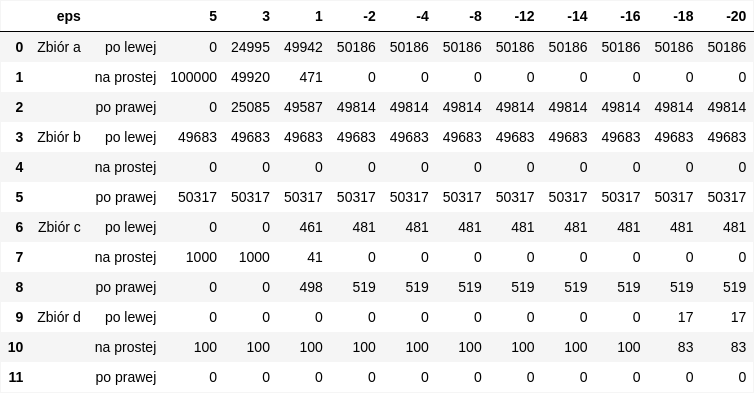
\includegraphics[scale=0.6]{eps_compar.png}
\subsection{Analiza wyników}
\begin{enumerate}
    \item W zbiorze $a$ dla $\varepsilon \leq 10^{-2}$ widzimy brak zmian 
w ilości zaklasyfikowanych do różnych zbiorów punktów. Także charakterystyczną dla tego $\varepsilon$ 
cechą można nazwać $0$ punktów rozpoznanych jako leżące na prostej.\\
Żeby zweryfikować nasze wyniki policzmy prawdopodobieństwo, że punkt w naszym zbiorze zostanie 
wylosowany w miejscu dla którego będzie zaklasyfikowany, jako należący do prostej. 
W naszych obliczeniach dla prostoty pominiemy niepewności związane z obliczeniami komputerowymi.\\
Klasyfikujemy punkty do odpowiedniej grupy obliczając iloczyn wektorowy
$\overrightarrow{ab} \times \overrightarrow{ac}$, gdzie $ c = (x,y)$ jest punktem, dla którego poszukujemy wiadomości o lokalizacji względem prostej przechodzącej przez punkty $ a$ i $ b$. Metoda ta jest równoznaczna z obliczeniem wyznacznika macierzy $ 2\times2$:  

$$
(1)\det(a, b, c)= \begin{vmatrix}
       a_{x} - c_{x} & a_{y} - c_{y} \\
       b_{x} - c_{x} & b_{y} - c_{y} 
              \end{vmatrix}.
$$\\
Wiemy także, że iloczyn wektorowy $\overrightarrow{A} \times \overrightarrow{B}$ można także obliczyć ze wzoru: 
$$
\overrightarrow{A} \times \overrightarrow{B} = ||A|| \cdot ||B|| \cdot \sin{\theta}.
$$
Gdzie $\sin{\theta}$ to kąt pomiędzy wektorami $\overrightarrow{A}$ i $\overrightarrow{B}$.\\
Wybierzmy teraz dla konkretnego punktu $c$ takie $a$ i $b$ na prostej, żeby 
\begin{enumerate}
    \item Dla $A = \overrightarrow{ab}, ||{A}|| = 1$.
    \item $\sin{\theta} = 1$, gdzie $\theta$ jest kątem pomiędzy $\overrightarrow{ab}$ i $\overrightarrow{ac}$ (wektor $\overrightarrow{ac}$ jest prostopadły do naszej prostej i do wektora $\overrightarrow{ab}$).
\end{enumerate}
Wtedy nasz iloczyn $$\overrightarrow{A} \times \overrightarrow{B} = ||A|| \cdot ||B|| = 1 \cdot ||B|| = ||B||.$$
I pytanie klasyfikacji punktu jako należacego do prostej sprowadza się do sprawdzenia czy $||B|| < \varepsilon$.
Dal zbioru $a$ długość prostej na całym zbiorze jest około 
\end{enumerate}